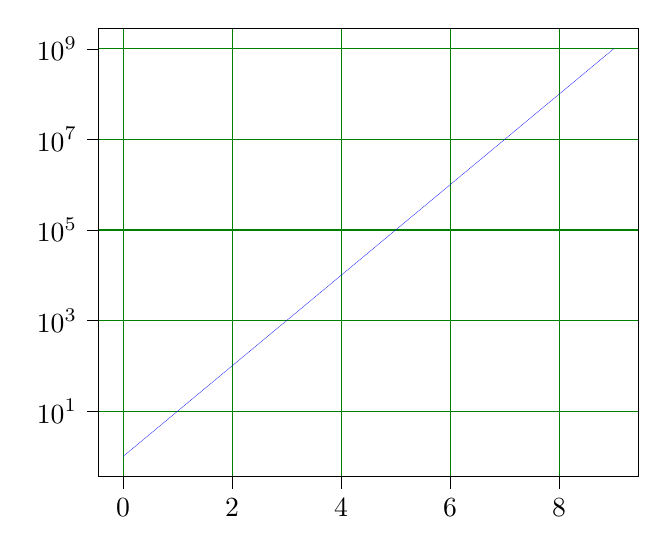
\begin{tikzpicture}

\definecolor{green01270}{RGB}{0,127,0}

\begin{axis}[
log basis y={10},
tick align=outside,
tick pos=left,
x grid style={green01270},
xmajorgrids,
xmin=-0.45, xmax=9.45,
xminorgrids,
xtick style={color=black},
y grid style={green01270},
ymajorgrids,
ymin=0.35481339, ymax=2.8183829e+09,
yminorgrids,
ymode=log,
ytick style={color=black},
ytick={0.001,0.1,10,1000,100000,10000000,1e+09,1e+11,1e+13},
yticklabels={
  \(\displaystyle {10^{-3}}\),
  \(\displaystyle {10^{-1}}\),
  \(\displaystyle {10^{1}}\),
  \(\displaystyle {10^{3}}\),
  \(\displaystyle {10^{5}}\),
  \(\displaystyle {10^{7}}\),
  \(\displaystyle {10^{9}}\),
  \(\displaystyle {10^{11}}\),
  \(\displaystyle {10^{13}}\)
}
]
\addplot [ultra thin, blue]
table {%
0 1
1 10
2 100
3 1000
4 10000
5 100000
6 1000000
7 10000000
8 1e+08
9 1e+09
};
\end{axis}

\end{tikzpicture}
